% Commented out: 
% \addbibresource
% \includepdf

\documentclass[12pt,letterpaper,english,bibliography=totocnumbered, abstract=on]{scrartcl}

\usepackage{indentfirst}
\usepackage[titletoc]{appendix}
%\usepackage[latin1]{inputenc}  % Enable direct input of special national characters
\usepackage[english]{babel}    % Language settings
\usepackage{lmodern}           % Enable Latin Modern fonts
\usepackage{color}
\usepackage{verbatim}
\usepackage[unicode=true,pdfusetitle,
bookmarks=true,bookmarksnumbered=false,bookmarksopen=false,
breaklinks=true,pdfborder={0 0 0},pdfborderstyle={},backref=false,colorlinks=true]
{hyperref}
\hypersetup{linkcolor=blue,citecolor=blue,urlcolor=blue}

\usepackage{booktabs}
\usepackage{multirow}
\usepackage{adjustbox}
\usepackage{threeparttable}
\usepackage[table]{xcolor}
\usepackage{csquotes}
\usepackage{soul} % for hiliting text: \hl

\usepackage[backend=biber, style=authoryear, maxbibnames=99, dashed=false]{biblatex}
\setlength\bibitemsep{2\itemsep}
\addbibresource{CASarticle.bib}
%\addbibresource{CRB.bib}

\usepackage{pdfpages}
\usepackage{float} % Allows use of H to place floats

\usepackage{pgfgantt}

\usepackage{framed}

\usepackage{array}

% Prevent page breaks within paragraphs
% https://tex.stackexchange.com/questions/21983/how-to-avoid-page-breaks-inside-paragraphs
\widowpenalties 1 10000

\begin{document}

\title{Biological Control of the Cycad Aulacaspis Scale, \textit{Aulacaspis yasumatsui}}

\author{Contributions by Aubrey Moore}

\maketitle
%\footnote{\url{https://github.com/aubreymoore/2020-FS-CRB-biocontrol-project/blob/master/combined-proposal.pdf}}
\newpage
\tableofcontents

\pagebreak

\section{Abstract - Cave}

\section{Introduction - Cave}

\section{Economic impact of CAS - Cave and Wright}
\section{Ecological impact of CAS - Moore}

Ecological impact of CAS invasions varies greatly with location, largely due to differences in characteristics of host plant populations, climate, and presence of natural enemies.

When CAS arrived in Florida (1995) and Hawaii (1998), it became a pest of ornamental cycads which could be protected using a combination of pesticide applications and biological control. 

However, when CAS arrived in Guam (2003), it rapidly spread from ornamental cycads, \textit{Cycas revoluta} and \textit{Cycas micronesica} to the wild \textit{Cycas micronesica} population, causing an uncontrolled island-wide outbreak. 

\paragraph{\textit{C. micronesica} taxonomy} \textit{Cycas micronesica} K. D. Hill 1994 is endemic to Micronesia currently growing on Guam, the Northern Mariana Islands, the Yap Islands, and the Palau Islands. Prior to its description of a new species \parencite{hillCycasRumphiiComplex1994}, it was identified as \textit{C. rumphii} or \textit{C. circinalis}.

\paragraph{Pre-invasion status of \textit{C. micronesica}}

At that time, \textit{C. micronesica} was the most abundant tree in Guam's forests \cite{donnegon_guams_2004}. \textit{C. micronesica} is endemic to Guam, the Northern Mariana Islands,Yap and Palau were it evolved tolerance to local abiotic threats such as typhoons and draught. 

In 2006, \textit{C. micronesica} was placed on the Red List of Threatened Species and in 2015 this plant was added to the US Endangered and Threatened Species List.

\paragraph{Invasive pathway for arrival of \textit{A. yasumatsui} on Guam} 

Arrival on of CAS on Guam was predicted. On February 13 2000 T. E. Marler published an article in the Gardening section of the Pacific Daily News entitled \textit{Looking out for scale insects} (\cite{haynesExoticInvasivePest2005}). Alarmed by establishment of CAS in Hawaii, Marler warned of pending arrival on Guam and pleaded for a ban cycad imports to the island. 

Both of the leading actors in this story are relatively new to science: \textit{Aulacaspis yasumatsui} described as an herbivore of cycads in Thailand \parencite{takagiNewSpeciesAulacaspis1977} and \textit{Cycas micronesica} K. D. Hill 1994 was described as a cycad species endemic to Micronesia \parencite{hillCycasRumphiiComplex1994}.

The Guam CAS outbreak was severe and rapid (Table 1).

\begin{table}[H]
	\centering
	\label{tab:timeline}	
	\caption{Timeline for the Guam CAS infestation.}	
	\begin{tabular}{l>{\raggedright\arraybackslash}p{4.5in}}
		\hline
		2000 & T. E. Marler predicts of arrival of CAS on Guam in a Pacific Daily News article \parencite{haynesExoticInvasivePest2005}\\
		\hline
		2002 & An initial US Forest Service survey indicates that \textit{C. micronesica} is Guam's most abundant tree (with stem diameter greater than 5 inches) and estimates a population size of 1,571,556 \parencite{donnegon_guams_2004}\\
		\hline
		2003 & CAS first detected on ornamental \textit{Cycas revoluta} and \textit{C. micronesica} at hotels in Tumon Bay  \\
		\hline
		2006 & \textit{C. micronesica} added to the IUCN Red List of Endangered and Threatened Species\\
		\hline
		2013 & A second US Forest Service survey ranks \textit{C. micronesica}, misidentified in the report as \textit{C. circinalis}, is Guam's xxrd most abundant tree (with stem diameter greater than 5 inches) and estimates a population size of n,nnn,nnn \parencite{lazaroGuamForestResources2020a}\\
		\hline
		2015 & \textit{C. micronesica} added to the US list\\
		\hline
	\end{tabular}	
\end{table}

CAS was first detected in the Tumon Beach hotel area of Guam near the end of 2003 on \textit{C. micronesica} and \textit{C. revoluta} growing as ornamental plants at two hotels. In those days, almost every hotel had cycad displays near their entrances.

It is likely that CAS arrived on Guam via importation of infested cycads from Hawaii, Florida or elsewhere. However, there are is no evidence that this occurred. There are no records of legal cycad importation to Guam in the two years prior to detection of CAS on the island (R. Campbell, Guam Plant Inspection Facility, personal communication).  

An intriguing possibility is that CAS arrived on Guam as crawlers. For many years there was an active infestation of CAS on \textit{C. revoluta} growing in an outdoor garden at the Honolulu International Airport located within a few hundred meters of where passengers boarded a daily 7.5 hour flight to Guam. Possibly crawlers were carried on clothing of passengers visiting this garden. Alternatively, airborne crawlers me have been blown into cargo holds or other spaces on Guam-bound aircraft.

\paragraph{History of the Guam CAS outbreak}

The trajectory and impact of the Guam CAS outbreak is well documented by T. E. Marler and others.

MAYBE A TABLE HERE?

\paragraph{Impact of CAS on the Guam \textit{C. micronesica} population}

\paragraph{Impact of CAS on \textit{C. micronesica} individuals}

Increased threat of island endemic tree?s
extirpation via invasion-induced decline of
intrinsic resistance to recurring tropical cyclones

Impacts to plants infested with CAS linger after the scale insects have been killed by insecticides or biocontrol agents. Scale covers block photosysnthesis \parencite{tangReportRecommendationsCycad2005a}.

Plants which have recovered from CAS infestation are structurally weakend and are susceptible to typhoon damage \parencite{marlerIncreasedThreatIsland2013}.

Plants which have recovered from CAS infestation are less able to reproduce \parencite{marlerAulacaspisYasumatsuiInvasion2021}, \parencite{marlerAulacaspisYasumatsuiInvasion2021},


\paragraph{Cascading impacts of CAS}

Effects on soil \cite{marlerTwoCycadSpecies2020}


\cite{haynesExoticInvasivePest2005}



\section{Natural enemies of CAS - Cave}

\section{Classical biological control}

\subsection{Florida - Cave}

\subsection{Hawaii - Wright}

\subsection{Guam - Moore}

\subsubsection{\textit{Rhyzobius lophanthae}}

About 100 adults of \textit{Rhyzobius lophanthae} were field collected on Maui and imported to Guam during November 2004. This coccinelid was originally 
introduced to California from Australia in 1892 and to Hawaii from California in 1894. It was observed feeding voraciously on CAS shortly after arrival of this new pest in Hawaii. 

\textit{R. lophanthae} was previously introduced to Guam on two separate occasions under various synonyms: \textit{R. satelles} Blackburn, \textit{Lindorus lophanthae} (Blaisdell), and \textit{R. pulchellus} Montrouzier (\cite{nafus_biological_1989}). 

In 1925 and 1926 Rhyzobius satelles was imported to Guam from California to control the coconut scale, \textit{Aspidiotus destructor} Signoret. However, attempts at field establishment failed.  

\cite{nafus_biological_1989} also report "In 1971, \textit{Rhyzobius satelles} Blackburn (as \textit{R. pulchellus} Montrouzier) was introduced to Guam from New Caledonia to aid in the control of coconut scales and citrus scales. A single specimen of \textit{R. satelles} was recovered in 1978, indicating establishment. The beetle, however, is very uncommon; an intensive survey of coconut insects in 1984 yielded no specimens."

The beetles from Maui were reared on scale-infested \textit{C. micronesica} cuttings placed in a large screened camping tent set up in a laboratory. Adult offspring were collected for field release by aspirating them from the walls of the tent into plasic vials. Field releases were initiated on February 16 2005 at the Guam National Wildlife Refuge at Ritidian Point. The beetles established readily. By July 7 2005 high densities on adults were observed on cycads anywhere within a 1 lm radius of the release site.  Establishment and dispersion of the beetles were monitored using yellow sticky traps deployed between June 2005 and May 2006. Unexpectedly, we were also able to monitor CAS crawlers and adult males using these traps (Fig. \ref{fig:sticky-traps})  (\cite{moore_biological_2017-2}). Following establishment of \textit{R. lophanthae} at Ritidian Point, laboratory-reared and field-collected beetles were released at about 30 other sites throughout Guam. 

\begin{figure}[H]
	\centering
	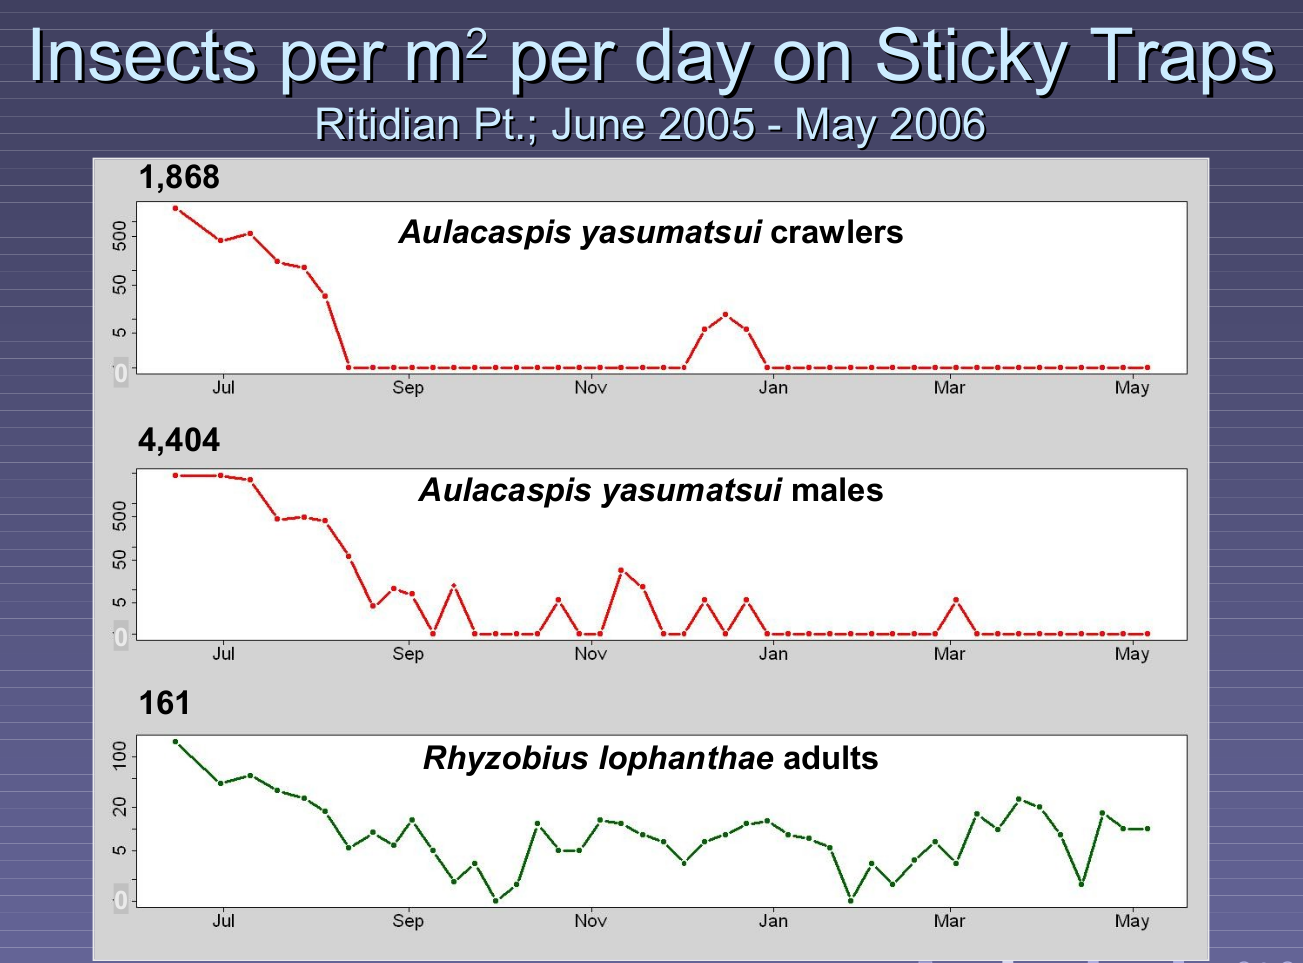
\includegraphics[width=0.7\linewidth]{sticky-traps}
	\caption{Caption goes here.}
	\label{fig:sticky-traps}
\end{figure}

By about 2010, \textit{R. lophanthae} larvae or adults could be found on almost every CAS-infested cycad on Guam, preventing CAS from killing mature cycads. By 2010, about 90\% of wild cycads had been killed on Guam (REF). Unfortunately, the \textit{C. micronesica} population is not recovering because almost all seeds and seedlings are being killed by CAS and other causes (REF). \cite{marlerVerticalStratificationPredation2013} showed that \textit{R. lophanthae} predation of CAS is significantly reduced close to the ground and suggest that this may partially account for failure of the beetle to protect CAS seedlings. They also suggested:
\begin{displayquote}
The causes of reduced scale predation by
\textit{R. lophanthae} near the ground are unknown,
but a parasitoid biological control agent may
not exhibit these same limitations. Furthermore, because a parasitoid would be much
smaller than \textit{R. lophanthae}, it would likely be
better able to access scale infestations within
cracks and crevices on \textit{C. micronesica} and
\textit{C. revoluta} trees.
\end{displayquote}

\subsubsection{\textit{Coccobius fulvus}}  

\subsubsection{\textit{Aphytis lignanensis}}

\subsubsection{\textit{Arrhenophagus}}  

Ask Mark, Janis about Bernarr's report on fortuitous introduction of CAS parasitoids.

Ask Reddy about his report.

Ask Arnold Harra.


\subsection{Elsewhere - Cave}

\section{Prospects for future action - Cave, Wright, and Moore}

\newpage
\printbibliography[heading=bibintoc]

\end{document}
